\documentclass[11pt,a4paper]{article}
\usepackage[utf8]{inputenc}
\usepackage[french]{babel}
\usepackage[T1]{fontenc}
\usepackage{amsmath}
\usepackage{amsfonts}
\usepackage{amssymb}
\usepackage{graphicx}
\usepackage{tikz}
\usepackage[left=2cm,right=2cm,top=2cm,bottom=2cm]{geometry}
\usepackage{hyperref}
\usepackage{float}
\usepackage{xcolor}
\usepackage{pgfplots}
\usepackage{asymptote}
\usepackage[european, straightvoltages, RPvoltages]{circuitikz}
\usetikzlibrary{babel}
\usepackage{siunitx}
\usepackage{wrapfig}
\usepackage{multicol} 
\usepackage{ulem}
\usepackage{listings}
\usepackage{schemabloc}
\setlength{\parindent}{0pt}

\title{PROJET EIS - PX222}
\author{Guillemot MOUSSU et Rémi MAZZONE}
\date{2° semestre - 2022-2023}

\begin{document}
\maketitle
\tableofcontents
\listoffigures
\pagebreak

\section{Séance 0 - 21/03/2023}
\subsection{Notes prises au tableau}
\begin{figure} [H]
\begin{center}
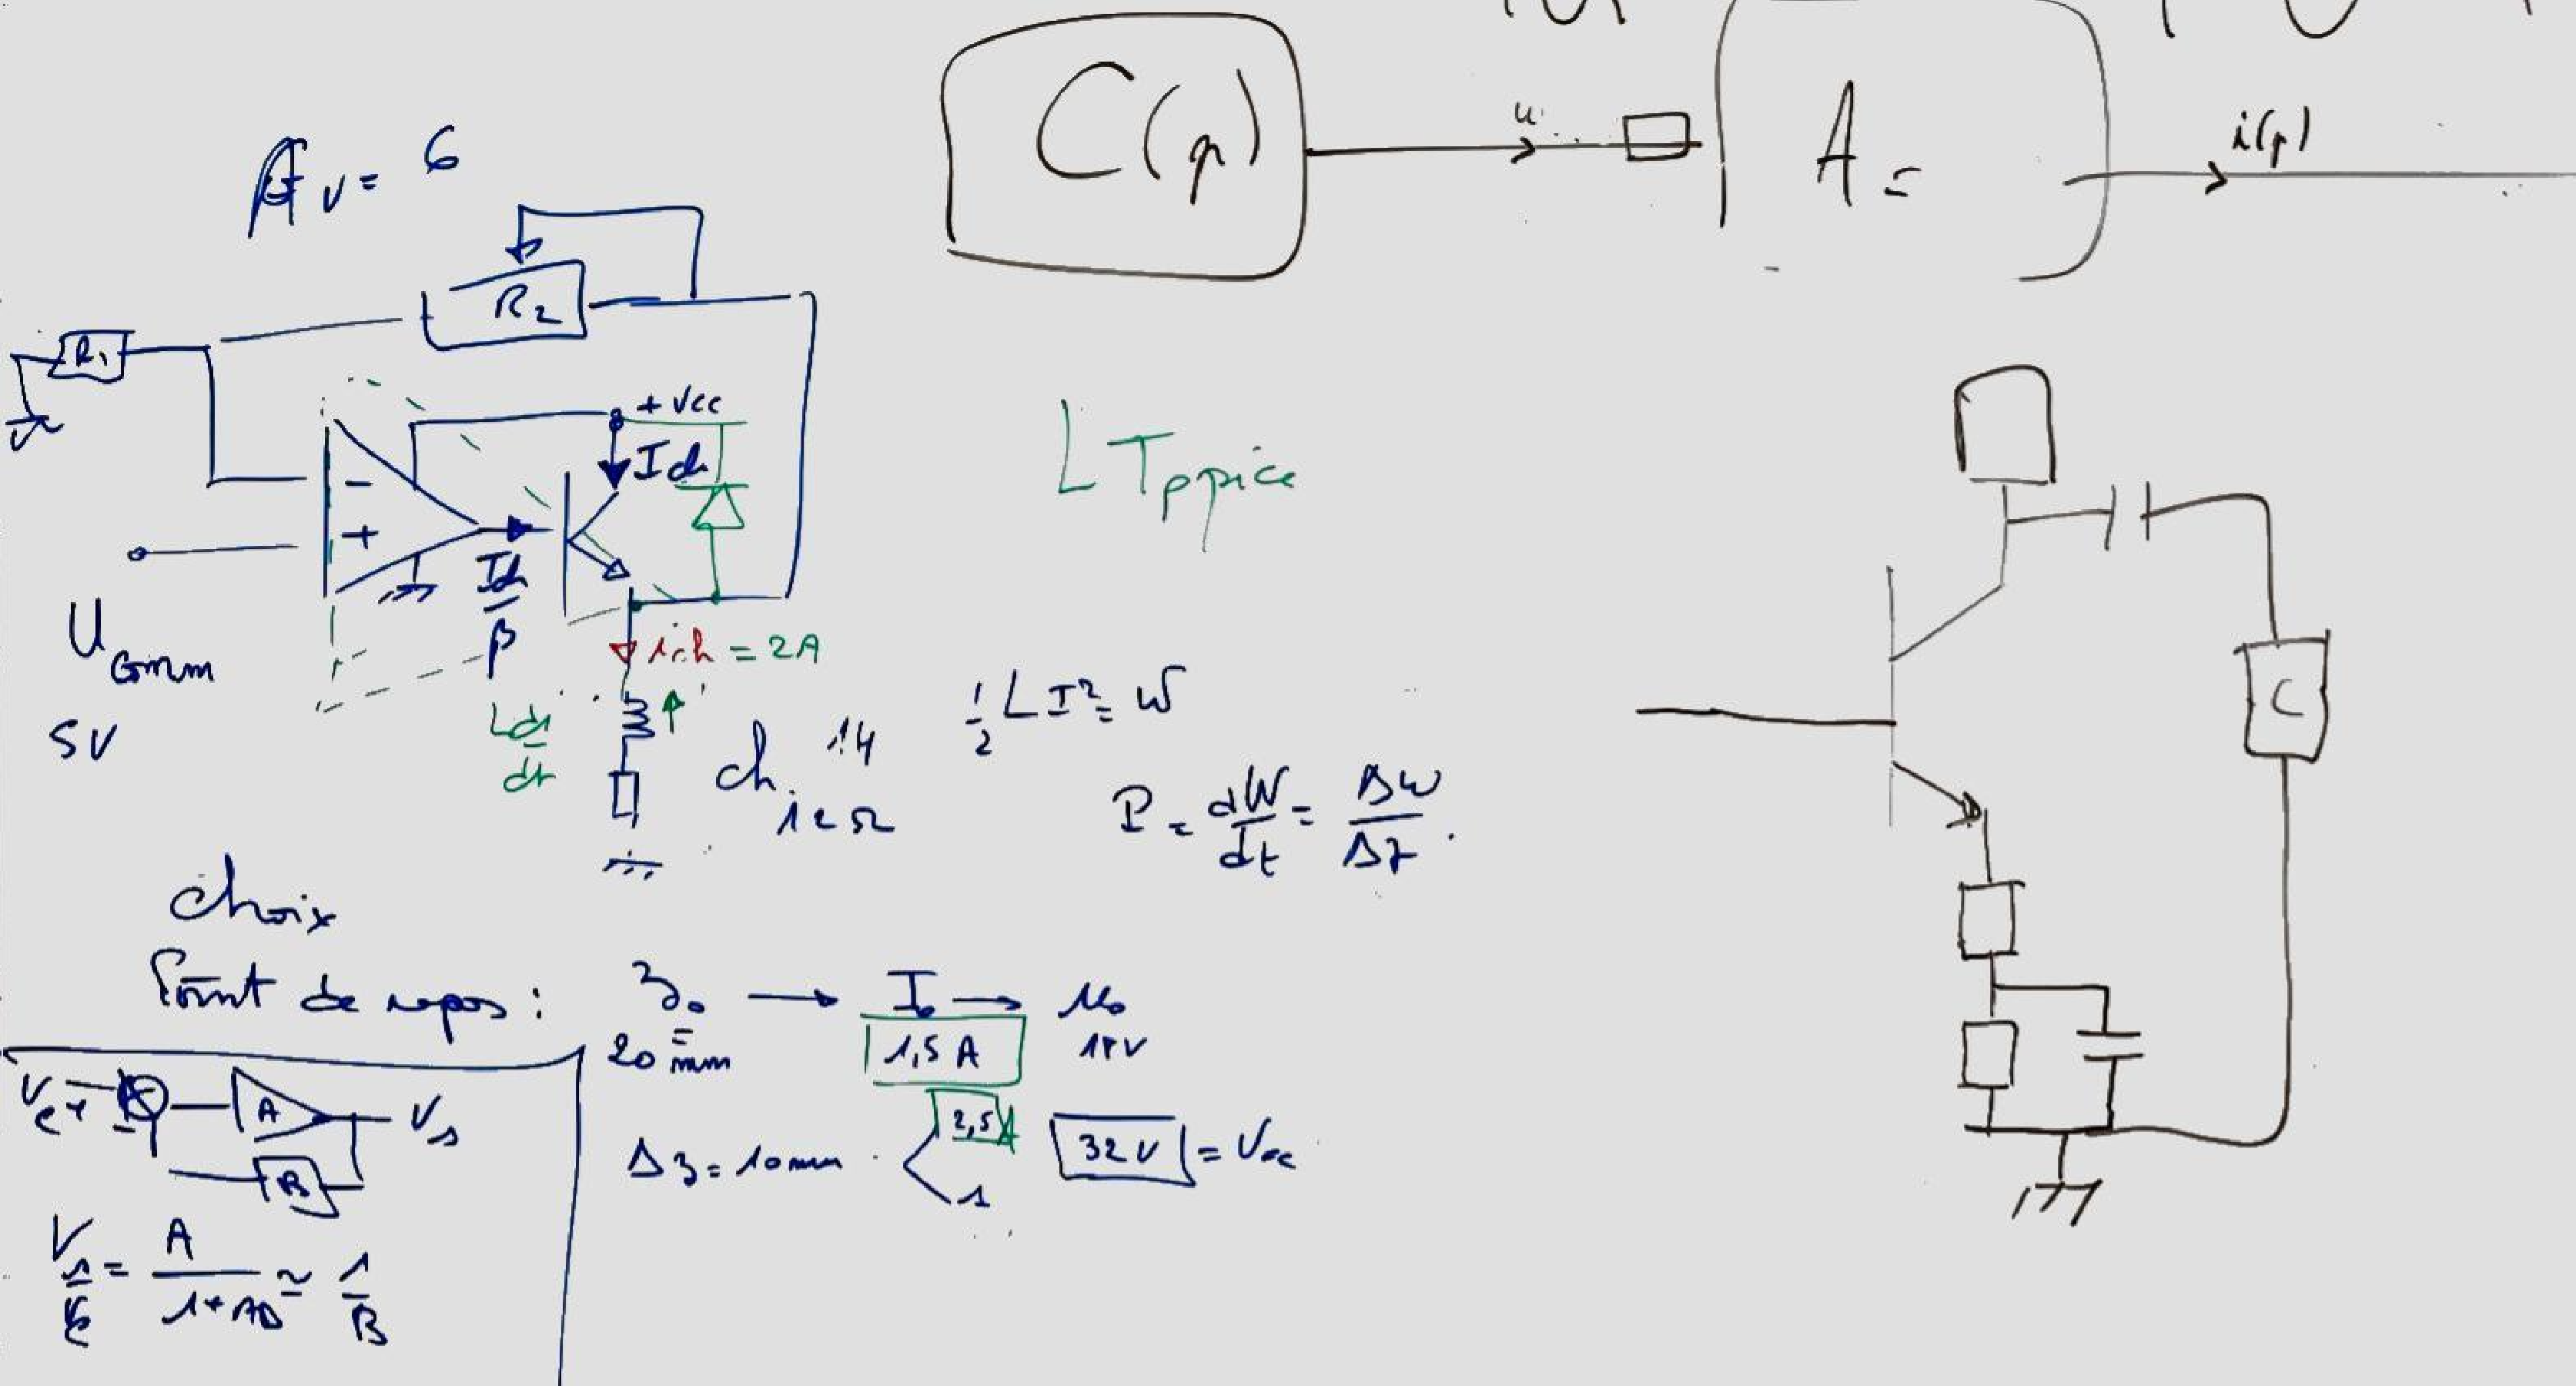
\includegraphics[width=0.9\textwidth]{Schémas/Notes tableau séance 0.png} 
\end{center}
\caption{Notes séance 0}
\end{figure}

\subsection{Idées de plan de recherches}
\begin{itemize}
\item \textbf{Caractérisation de la bobine} : mesure de la résistance et l'inductance de la bobine. Cela permettra de modéliser la bobine et de calculer le champ magnétique qu'elle produit
\item \textbf{Modélisation de la bobine} : utilisation des valeurs mesurées pour construire un modèle électrique de la bobine, par exemple en utilisant l'équation de l'inductance d'une bobine. Pour une précision plus élevée, il peut être nécessaire d'inclure d'autres effets tels que la saturation du noyau de la bobine ou la résistance série équivalente
\item \textbf{Étude du champ magnétique de la bobine} : calcul de la distribution du champ magnétique à l'aide d'un logiciel de simulation. Validation des résultats expérimentalement
\item \textbf{Choix d'un capteur de distance} : choix d'un capteur de distance infrarouge adapté à la plage de mesure et à la précision requises. La fréquence de mesure et la plage de mesure peuvent influencer le résultat
\item \textbf{Calibration du capteur de distance} : déterminer la relation entre la tension de sortie du capteur et la distance de la bille par rapport à la bobine
\item \textbf{Conception d'un correcteur } : utiliser les données obtenues précédemment pour concevoir un correcteur proportionnel-intégral-dérivé (PID) ou un correcteur à avance de phase pour contrôler la position de la bille. C'est la partie clé de ce projet. Le correcteur PID est une méthode de contrôle classique qui est souvent utilisée pour les systèmes de positionnement. Un correcteur à avance de phase peut également être utilisé pour améliorer les performances.
\item \textbf{Implémentation du correcteur } : test du correcteur via Matlab et Simulink
\item \textbf{Étalonnage du système} : ajuster les paramètres du correcteur pour atteindre la précision et la stabilité requises
\item \textbf{Validation du système} : tester le système dans différentes conditions et valider ses performances
\item \textbf{Optimisation du système} : améliorer le système en optimisant les paramètres du correcteur et en utilisant des techniques avancées de contrôle, telles que le contrôle prédictif et le contrôle adaptatif
\end{itemize}
\medskip
Il est important de noter que certains des points ont déjà été réalisés lors du premier semestre

\pagebreak
\section{Séance 1 - 05/04/2023}
\subsection{Reprise des éléments du semestre précédent}
Avec Hopkinson, nous avions obtenu un schéma équivalent de la bobine : 
\begin{figure}[H]
\begin{center}
\begin{circuitikz}
\draw
(0,0) to [V=$\varepsilon$] (0,2)
(0,2) to [short, i=$\varphi$] (2,2)
(2,2) to [R, l=$\mathfrak{R}_1$] (2,0)
(2,0) to [short] (0,0)
(2,2) to [R, l=$\mathfrak{R}(z)$, *-] (5,2)
(2,0) to [R, l=$\mathfrak{R}_0$, *-] (5,0)
(5,2) to [short] (5,0);
\end{circuitikz}
\caption{Modélisation de la bobine}
\end{center}
\end{figure}

Nous avions trouvé que la fonction de transfert de la bobine est : $\boxed{T_{BO}=\dfrac{Z}{I}=\dfrac{k_i}{k_z-mp^2}}$\\
Avec les valeurs suivantes :\\
\medskip
$I_0 = 2A$, $Z_0 = 22mm$, $L_1 = 6.73H$, $\alpha = 2.06$, $m = 35.8g$\\
$k_i = \dfrac{I_0 \cdot L_1 \cdot \alpha}{(1 + \alpha \cdot Z_0)^2}$, $k_z = \dfrac{I_0^2 \cdot L_1 \cdot \alpha^2}{(1 + \alpha \cdot Z_0)^3}$

\subsection{Utilisation de Matlab}
\label{Matlab1}
Nous avons donc notre fonction de transfert. Une idée qui nous est venue est d'adapter les scripts pour utiliser l'outil de M. Mendes que nous avons découvert en TP. Cela devrait nous permettre de calculer notre correcteur. Pour commencer, on a placé nos valeurs dans Matlab et tracé le bode obtenu. Cette étape est présente seulement pour nous faire une idée du système à l'heure actuelle

\begin{figure}[H]
Code Matlab que nous avons utilisé :
\begin{lstlisting}[language=Matlab]
I0 = 2;
Z0 = 22 * 10^-3;
L1 = 6.73;
alpha = 2.06;
ki = (I0 * L1 * alpha) / (1 + alpha * Z0) ^2;
kz = -(I0 ^2 * L1 * alpha ^2) / (1 + alpha * Z0) ^3;
m = 35.8;

num =  ki ;
den = [(-m) 0 kz];
sys = tf(num,den);

figure;
bode(sys)
grid on
figure;
nyquist(sys)
grid on
\end{lstlisting}
\end{figure}

\pagebreak
On obtient donc le bode suivant :
\begin{figure} [H]
\begin{center}
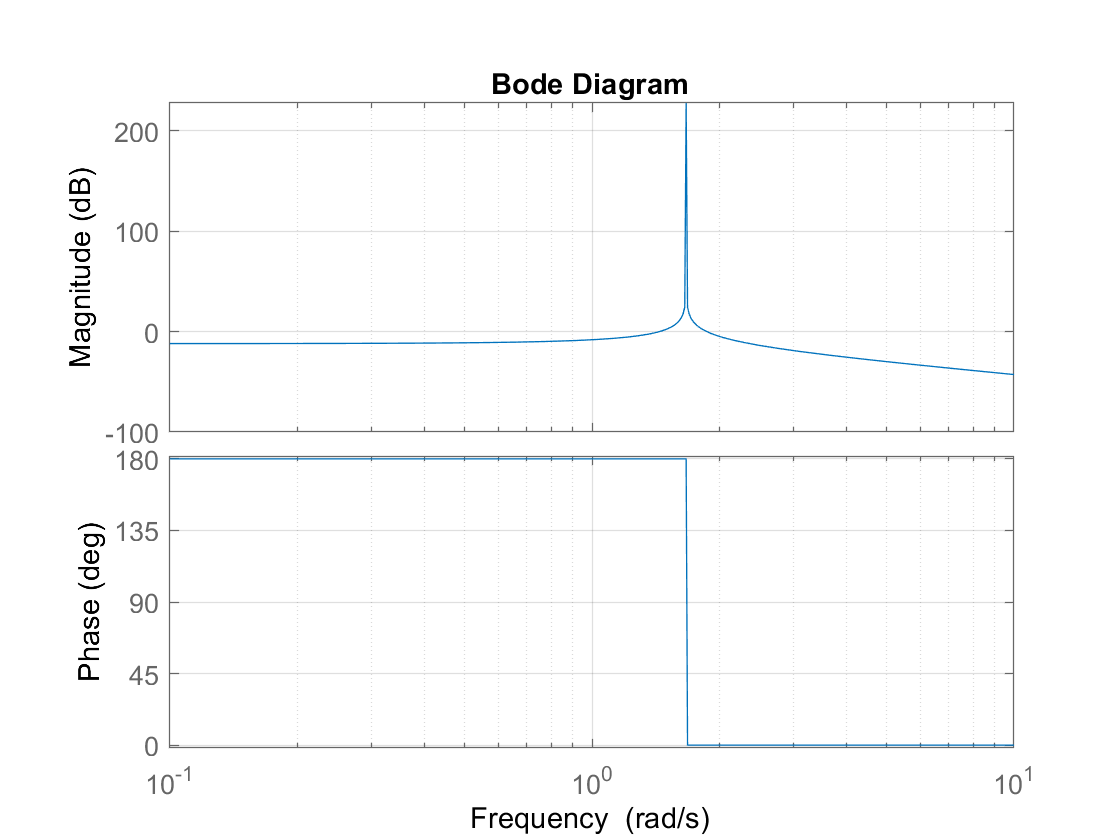
\includegraphics[width=0.9\textwidth]{Schémas/Bode initial.png} 
\end{center}
\caption{Bode obtenu}
\label{fig:Bode initial}
\end{figure}

On trace ensuite le diagramme de Nyquist :
\begin{figure} [H]
\begin{center}
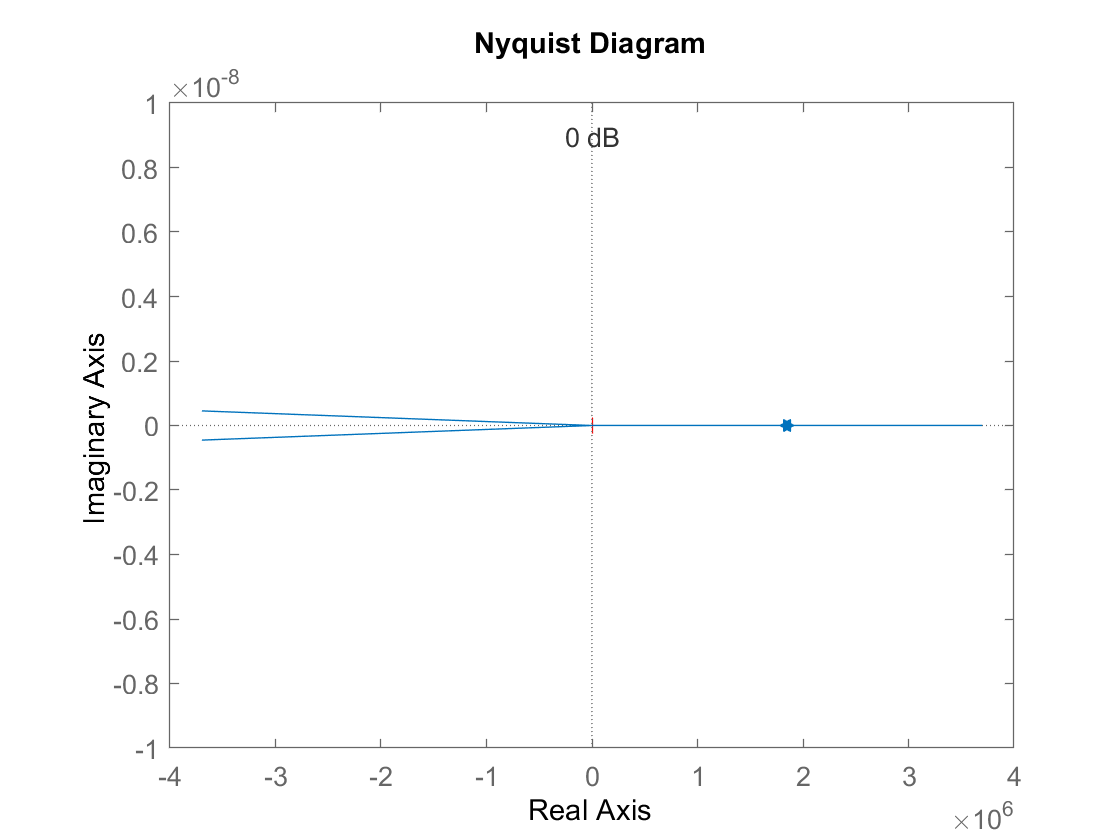
\includegraphics[width=0.6\textwidth]{Schémas/Nyquist initial.png} 
\end{center}
\caption{Nyquist obtenu}
\label{fig:Nyquist initial}
\end{figure}

On remarque donc qu'il reste du travail avant d'avoir un résultat satisfaisant, mais nous reviendrons sur ce point ultérieurement

\subsection{Modélisation point par point du système}
\label{Modélisation point par point}
L'objectif est de réaliser un circuit correspondant à ce schéma bloc :

\begin{figure} [H]
\begin{center}
\begin{tikzpicture}
\sbEntree{E}
\sbSumb{comp}{E}                
\sbRelier[$C$]{E}{comp}
\sbBloc{reg}{$R$}{comp}  
\sbRelier[$\varepsilon$]{comp}{reg}
\sbBloc{amp}{$A$}{reg}
\sbRelier[$U$]{reg}{amp}
\sbBloc{sys}{$H$}{amp}      
\sbRelier[$X$]{amp}{sys}
\sbSortie{S}{sys}                
\sbRelier[$Y$]{sys}{S}
\sbDecaleNoeudy[4]{S}{U}
\sbBlocr{cap}{$B$}{U}        
\sbRelieryx{sys-S}{cap}
\sbRelierxy[$Y_m$]{cap}{comp}
\end{tikzpicture}
\end{center}
\caption{Schéma bloc du système}
\label{fig:Schéma bloc}
\end{figure}

\subsubsection{Modélisation de l'amplificateur}
\label{Modélisation ampli}
Nous avons en sortie d'un STM8 un signal de 5V, nous voulons que la bobine soit alimentée en 30V. Pour cela on utilise un amplificateur à AOP, en série avec un transistor bipolaire. On a le schéma classique d'un amplificateur à AOP :

\begin{figure} [H]
\begin{center}
\begin{tikzpicture}
% Schéma bloc
\sbEntree{E}
\sbBloc{amp}{$A$}{E}
\sbRelier[$U$]{E}{amp}
\sbSortie{S}{amp}
\sbRelier[$X$]{amp}{S}

% Flèche entre les deux schémas
\draw[->, thick] (4,0) -- (6,0);

% Schéma elec
\draw (11,0) node[op amp] (opamp) {};
\draw (opamp.-) to[R, l=$R_1$] ++(-2,0) node[ground] {};
\draw (opamp.+) to[short, -*] ++(-0.5,0) node[label=left:$U$] {};
\draw (opamp.-) to[short] ++(0,1) coordinate (feedback);
\draw (feedback) to[R, l=$R_2$] ++(2,0) -| (opamp.out);
\draw (opamp.out) to[short, -o] ++(1,0) node[label=right:$X$] {};
\end{tikzpicture}
\end{center}
\caption{Amplificateur à AOP}
\label{fig:Amplificateur à AOP}
\end{figure}

Si on ajoute le transistor et la bobine au schéma, cela nous donne :
\begin{figure} [H]
\begin{center}
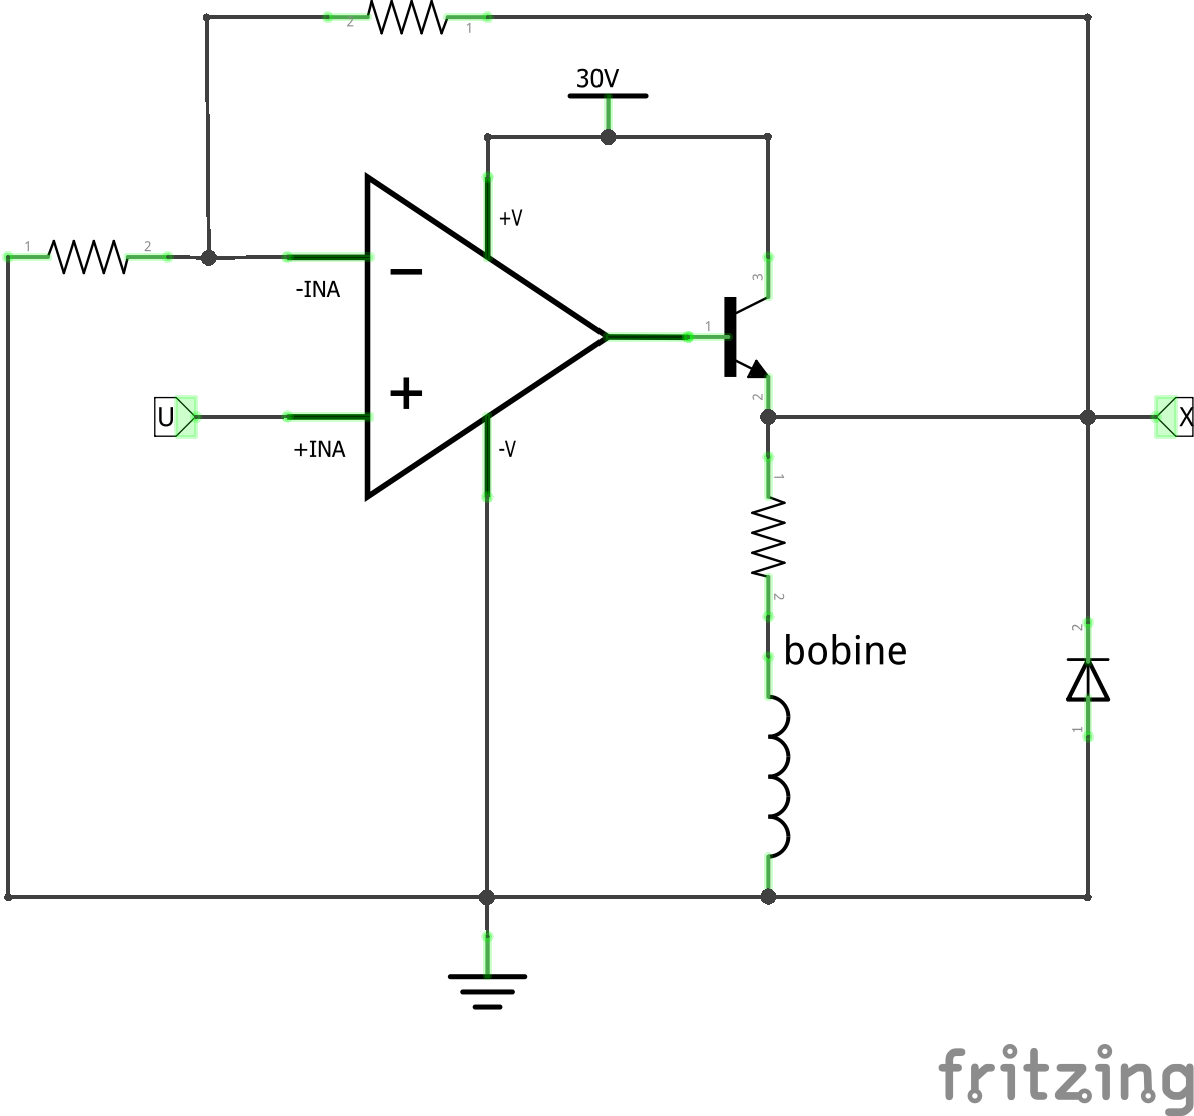
\includegraphics[width=0.6\textwidth]{Schémas/Ampli.png} 
\end{center}
\caption{Modélisation du bloc amplificateur}
\label{fig:Modélisation du bloc amplificateur}
\end{figure}

\subsubsection{Modélisation d'un régulateur PD}
\label{Modélisation PD}
On a le schéma classique d'un régulateur PD :

\begin{figure} [H]
\begin{center}
\begin{tikzpicture}
% Schéma bloc
\sbEntree{E}
\sbBloc{amp}{$R$}{E}
\sbRelier[$\varepsilon$]{E}{amp}
\sbSortie{S}{amp}
\sbRelier[$U$]{amp}{S}

% Flèche entre les deux schémas
\draw[->, thick] (4,0) -- (6,0);

% Schéma elec
\draw (11,0) node[op amp] (opamp) {};
\draw (opamp.-) to[R, l=$R_1$] ++(-2,0) coordinate (entry) {};
\draw (entry) to [short, -o] ++(-0.5,0) node[label=left:$\varepsilon$] {};
\draw (entry) to[short] ++(0,1) coordinate (pointC);
\draw (pointC) to [C, l=$C$] ++(2,0) -| (opamp.-);
\draw (opamp.+) to[short, -] ++(-0.5,0) node[ground] {};
\draw (opamp.-) to[short] ++(0,1) coordinate (feedback);
\draw (feedback) to[R, l=$R_2$] ++(2,0) -| (opamp.out);
\draw (opamp.out) to[short, -o] ++(1,0) node[label=right:$U$] {};
\end{tikzpicture}
\end{center}
\caption{Régulateur PD}
\label{fig:Régulateur PD}
\end{figure}

Si on donne le schéma complet de ce bloc, cela nous donne :

\begin{figure} [H]
\begin{center}
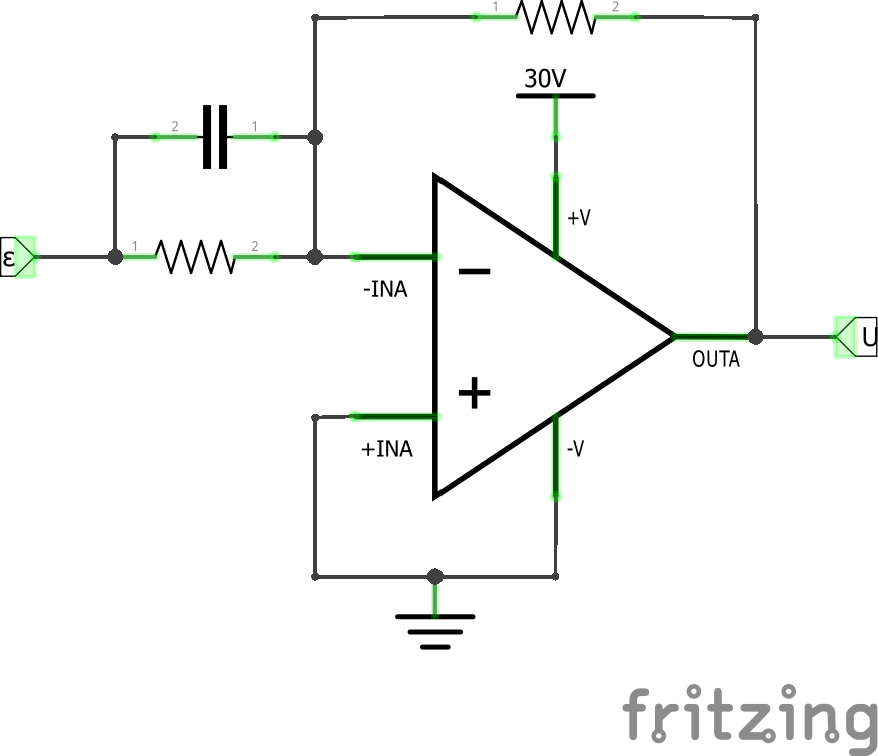
\includegraphics[width=0.5\textwidth]{Schémas/Correcteur PD.png} 
\end{center}
\caption{Modélisation du bloc régulateur (PD)}
\label{fig:Modélisation du bloc régulateur (PD)}
\end{figure}

\subsubsection{Modélisation d'un régulateur PID}
\label{Modélisation PID}
Dans le cas où l'on souhaite finalement modéliser un régulateur PID, on doit ajouter un condensateur en parallèle de notre résistance :

\begin{figure} [H]
\begin{center}
\begin{circuitikz}
\draw (0,0) node[op amp] (opamp) {};
\draw (opamp.-) to[R, l=$R_1$] ++(-2,0) coordinate (entry) {};
\draw (entry) to [short, -o] ++(-0.5,0) node[label=left:$\varepsilon$] {};
\draw (entry) to[short] ++(0,1) coordinate (pointC);
\draw (pointC) to [C, l=$C_1$] ++(2,0) -| (opamp.-);
\draw (opamp.+) to[short, -] ++(-0.5,0) node[ground] {};
\draw (opamp.-) to[short] ++(0,1) coordinate (feedback);
\draw (opamp.-) to[short] ++(0,2.5) coordinate (feedback2);
\draw (feedback) to[R, l=$R_2$] ++(2,0) -| (opamp.out);
\draw (feedback2) to[C, l=$C_2$] ++(2,0) -| (opamp.out);
\draw (opamp.out) to[short, -o] ++(1,0) node[label=right:$U$] {};
\end{circuitikz}
\end{center}
\caption{Régulateur PID}
\label{fig:Régulateur PID}
\end{figure}

\subsubsection{Modélisation du système complet (PD)}
\label{Modélisation complète}
On choisit le régulateur PD pour représenter le système complet. On a vu qu'il suffira d'ajouter une capacité pour passer à un régulateur PID au besoin. On repère bien les blocs comparateur, amplificateur et régulateur

\begin{figure} [H]
\begin{center}
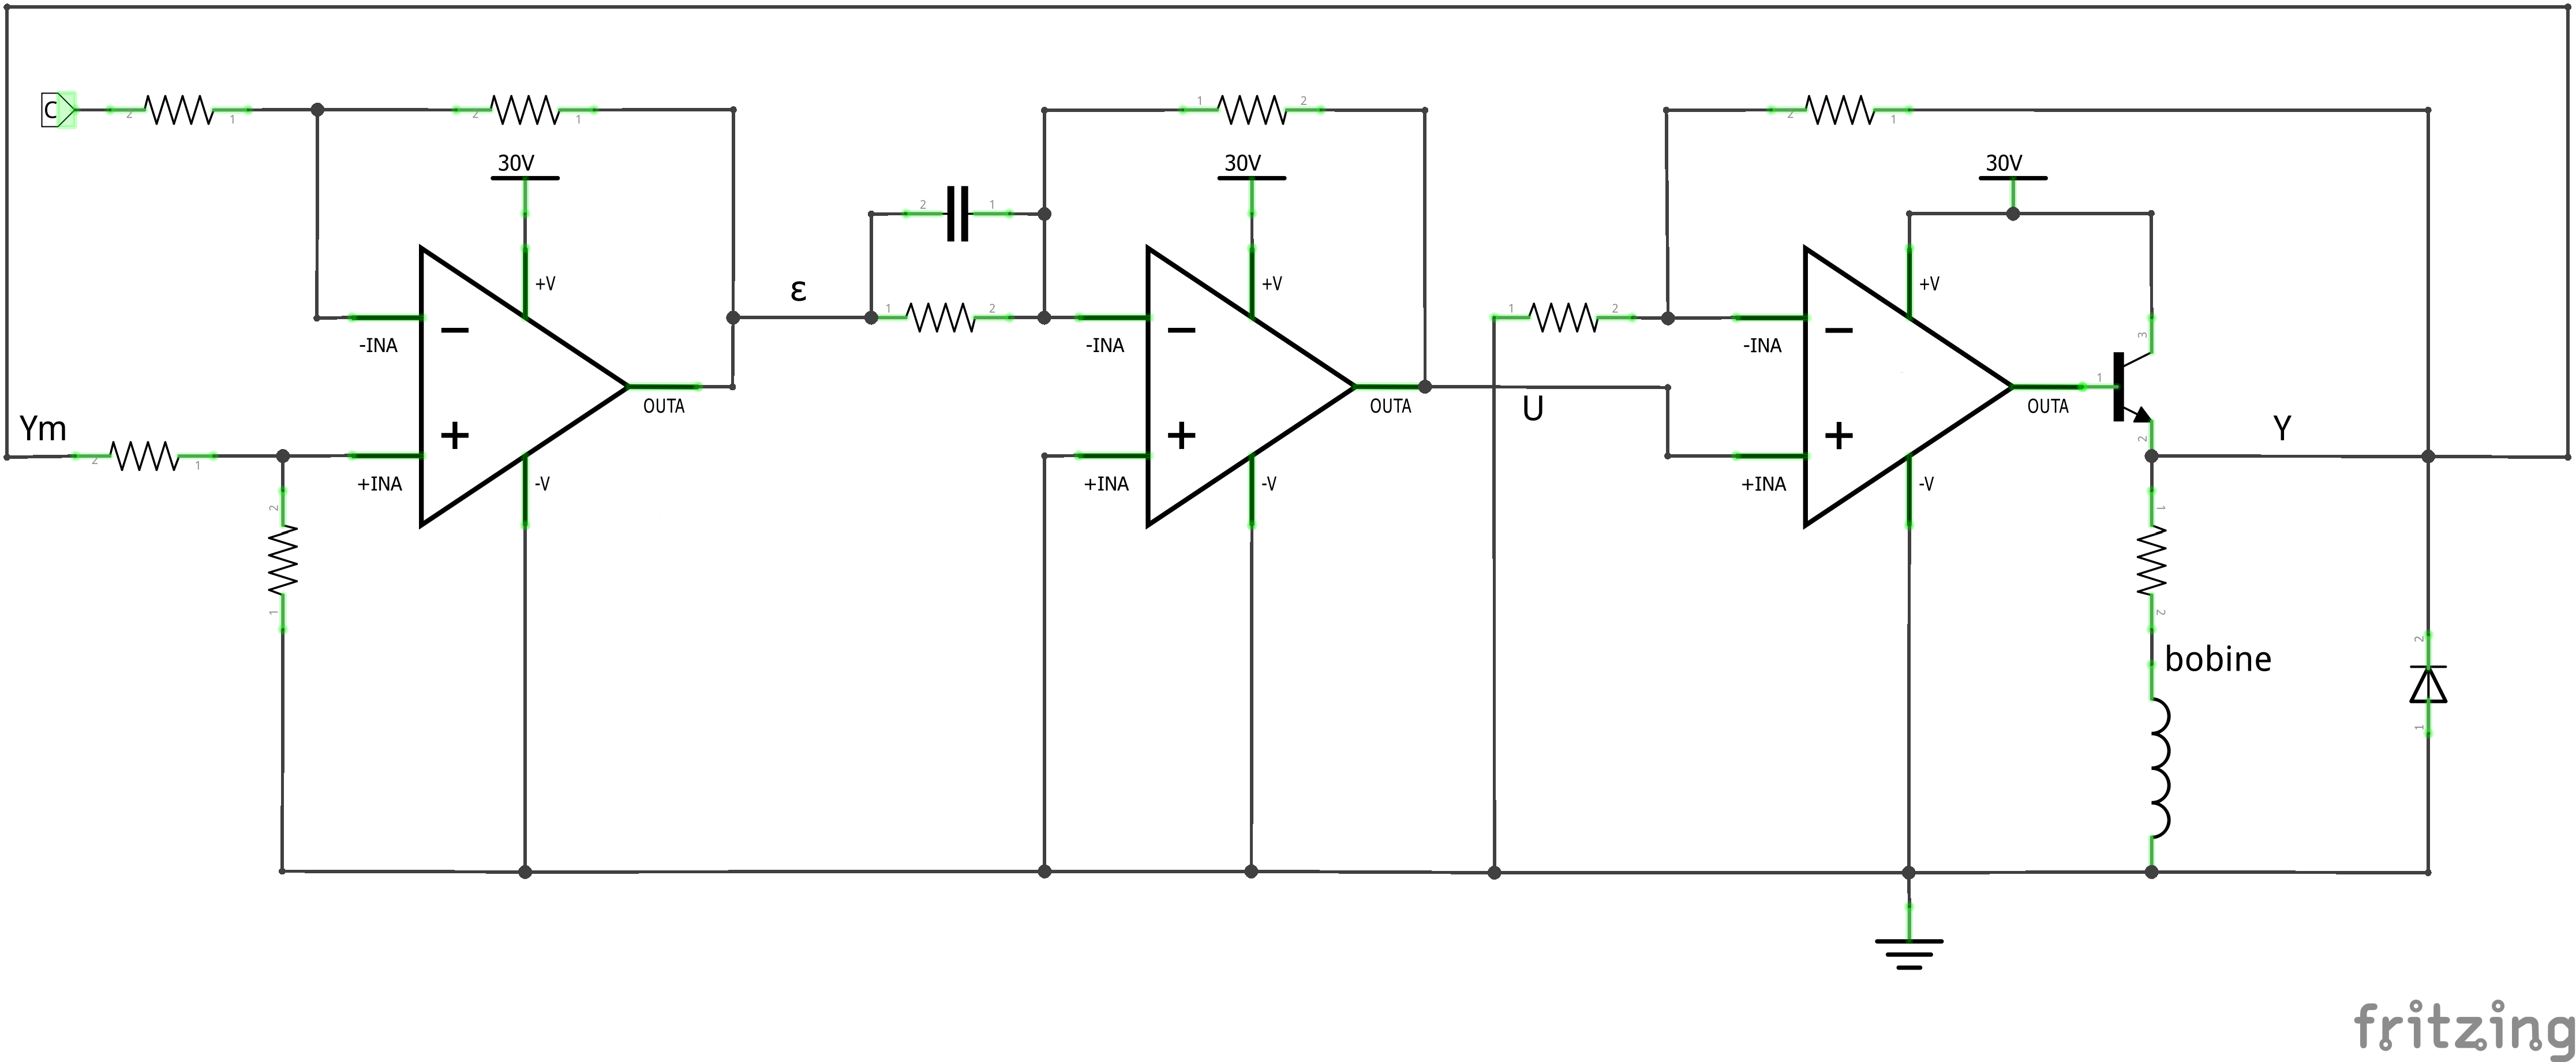
\includegraphics[width=1\textwidth]{Schémas/Modèle complet PD.png} 
\end{center}
\caption{Modélisation complète avec retour (PD)}
\label{fig:Modélisation complète avec retour (PD)}
\end{figure}


\subsection{Conclusions pour cette séance}
On commence à avoir des pistes intéressantes. Les schémas que nous avons réalisés vont nous permettre de se faire une idée du système à concevoir, et nous avons perçu l'importance d'utiliser Matlab pour nous aider dans nos calculs

\section{Travail entre les séance 1 et 2}
\subsection{Correction des éléments de la séance précédente}
Nous avions manqué de temps pour terminer comme nous le souhaitions certains points de la séance précédente. Nous avons travaillé sur les points suivants :
\subsubsection{Matlab}
\textit{Pour plus de détails se référer à la section} \ref{Matlab1}\\

Les schémas avaient étés rendus avec Octave, mais après comparaison des rendus, ceux de Matbab donnent d'autres résultats. Les figures \ref{fig:Bode initial} et \ref{fig:Nyquist initial} ont donc été mises à jour

\subsubsection{Modélisation point par point du système}
\textit{Pour plus de détails se référer à la section} \ref{Modélisation point par point}\\

La figure \ref{fig:Schéma bloc} est maintenant rendue en \LaTeX\\

Pour plus de clarté, les points \ref{Modélisation ampli}, \ref{Modélisation PD} et \ref{Modélisation PID} ont été repris. Les figures \ref{fig:Amplificateur à AOP}, \ref{fig:Régulateur PD} et \ref{fig:Régulateur PID} ont été reprises en \LaTeX. Les figures \ref{fig:Modélisation du bloc amplificateur} et \ref{fig:Modélisation du bloc régulateur (PD)} ont été reprises sur Fritzing, avec un bloc AOP mis à jour\\

Le point \ref{Modélisation complète} a été séparé plus plus de clarté. La figure \ref{fig:Modélisation complète avec retour (PD)} y a été ajoutée

\subsection{Simulation de l'amplificateur}
\begin{multicols}{2}
On veut donc simuler notre bloc amplificateur. Dans l'idéal on devrait avoir le graphique suivant :
\begin{figure} [H]
\begin{center}
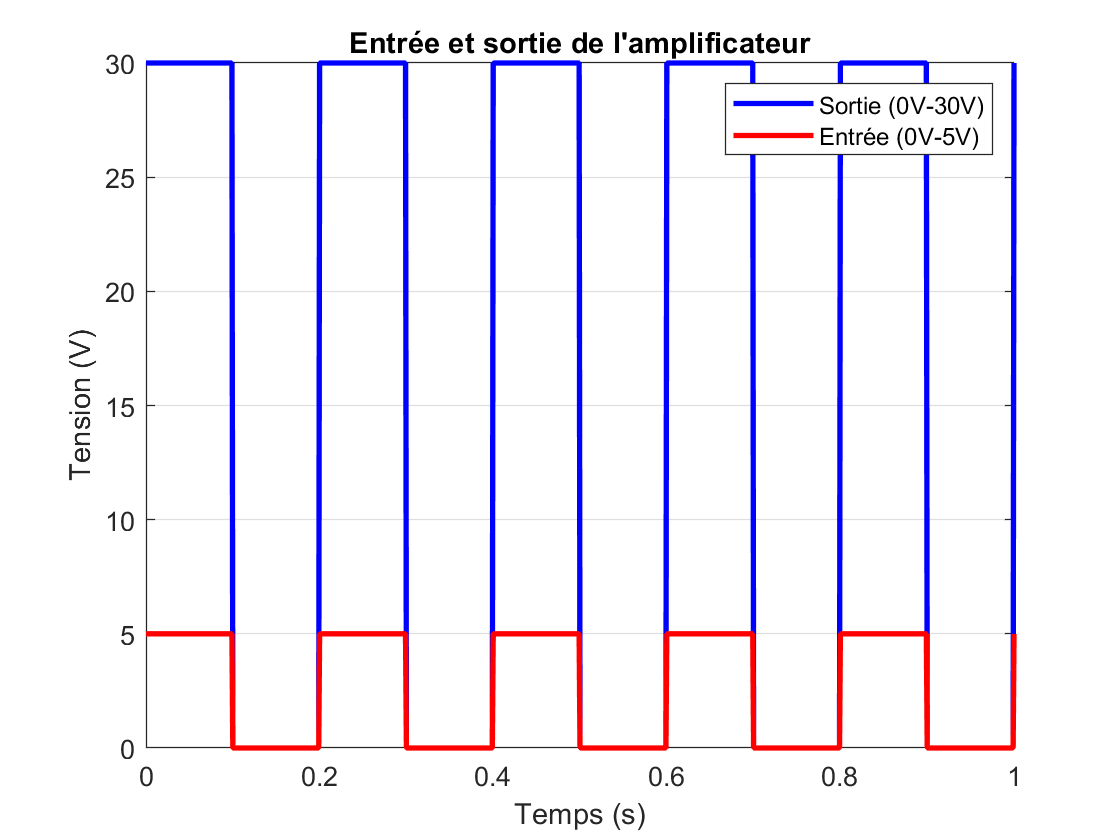
\includegraphics[width=0.5\textwidth]{Schémas/sim matlab ampli.png} 
\end{center}
\caption{Résulat idéal de la simulation}
\end{figure}

On rentre donc le modèle suivant dans LTSPICE :
\begin{figure} [H]
\begin{center}
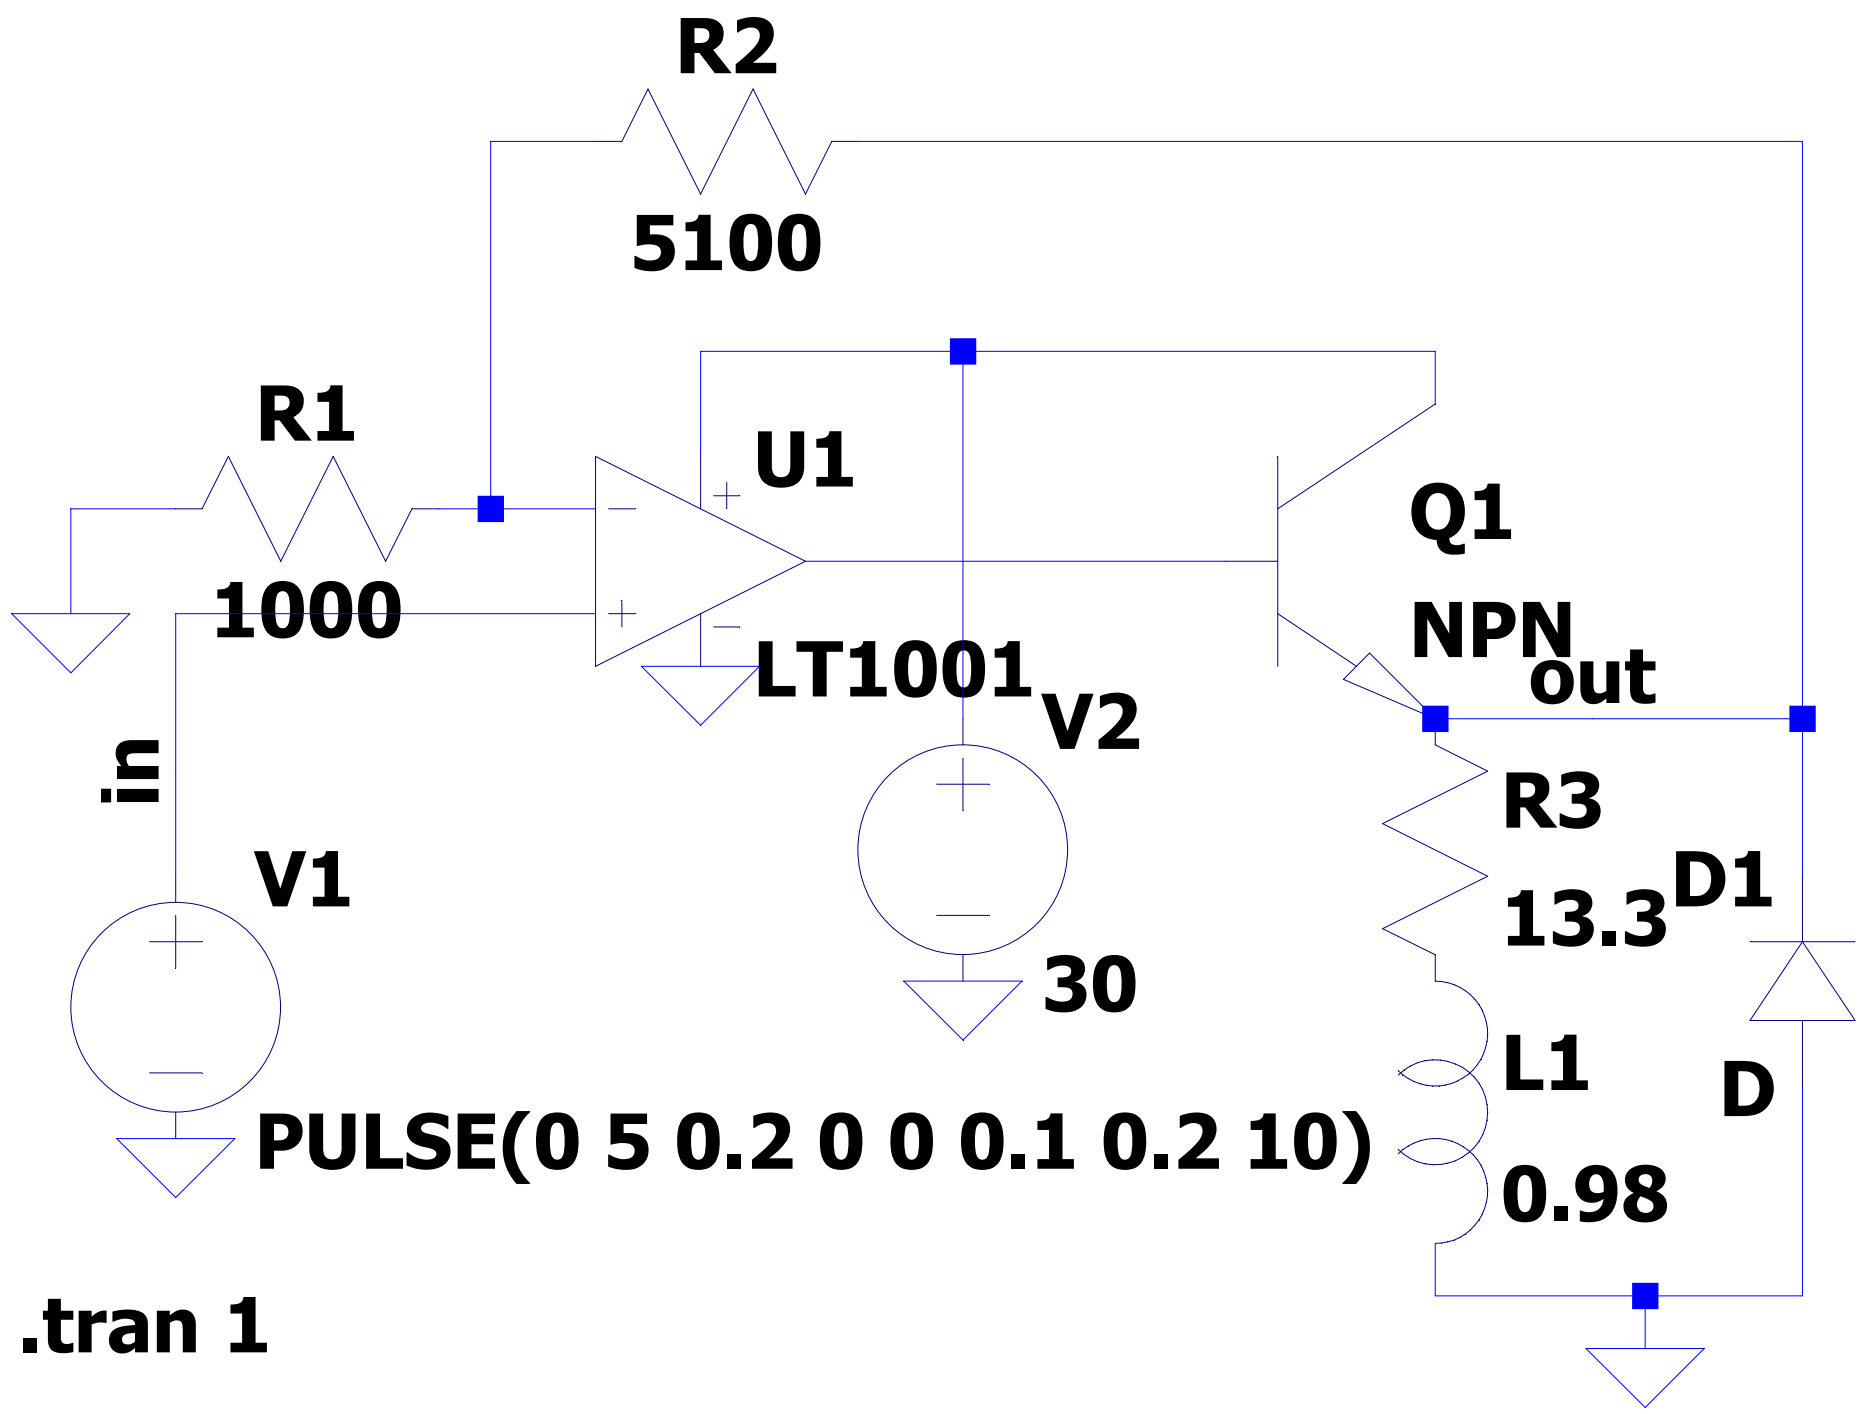
\includegraphics[width=0.5\textwidth]{Schémas/ltspice ampli.png} 
\end{center}
\caption{Schéma LTSPICE de l'amplificateur}
\end{figure}
\end{multicols}

Et on obtient le résultat suivant :
\begin{figure} [H]
\begin{center}
\includegraphics[width=1\textwidth]{Schémas/sim ampli.png} 
\end{center}
\caption{Simulation de l'amplificateur}
\end{figure}

\textbf{Remarques} :
\begin{itemize}
\item On a utilisé un AOP quelconque (le LT1001 en l'occurence)
\item On a utilisé les mesures de la bobine du S1 ($R=13.3\Omega$ et $L=0.98H$)
\item On a utilisé un transistor quelconque
\end{itemize}

On remarque que la simulation correspond au modèle théorique voulu. C'est bon signe pour la suite, il reste à le tester avec des composants réels

\pagebreak
\section{Bibliographie}
Liste des sites utilisés pour la réalisation du projet :
\begin{itemize}
\item \href{https://www.overleaf.com/learn}{Overleaf, guide d'utilisation du \LaTeX{}}
\item \href{https://chat.openai.com/chat}{ChatGPT, modèle de langage automatisé}
\item \href{https://ctan.mines-albi.fr/graphics/pgf/contrib/circuitikz/doc/circuitikzmanual.pdf}{Manuel de Circuitikz}
\end{itemize}

\end{document}